\documentclass[11pt]{article}
%%%%%%%%%%%%%%%%%%%%%%%%%%%%%%%%%%%%%%%%%%%%%%%%%%%%%%%%%%%%%%%
% DO NOT EDIT THIS FILE UNLESS YOU KNOW WHAT YOU ARE DOING!!! %
%%%%%%%%%%%%%%%%%%%%%%%%%%%%%%%%%%%%%%%%%%%%%%%%%%%%%%%%%%%%%%%

% Useful packages
\usepackage[]{authblk}
\usepackage{graphicx}
\usepackage{color}
\usepackage{longtable}
\usepackage{hanging}
\usepackage{indentfirst}
\usepackage{setspace}
\usepackage{enumitem}
\usepackage{verbatim}
\usepackage{upgreek}
\usepackage{framed}
\usepackage{textcomp}
\usepackage{url}
\usepackage{soul}
\usepackage{amsmath,amsfonts,amssymb,mathrsfs}
\usepackage{fancyhdr}
\usepackage[compact]{titlesec}
\usepackage[T1]{fontenc}
\usepackage{lmodern}
\usepackage[utf8]{inputenc}
\usepackage[]{listings}
%\usepackage{fontspec}
\usepackage{placeins}
\usepackage{epstopdf}
\usepackage[export]{adjustbox}
\usepackage{tikz}
\usepackage[breaklinks]{hyperref}
\usepackage[all]{hypcap}


% References
\usepackage[backend=bibtex,hyperref=true,citestyle=authoryear,bibstyle=authortitle,firstinits=true,terseinits=true,doi=false,url=false,eprint=false,maxbibnames=10,maxcitenames=2]{biblatex}
\input{biblatex_macros}

% Page margins
\setlength{\evensidemargin}{0in}
\setlength{\headheight}{0in}
\setlength{\headsep}{0in}
\setlength{\oddsidemargin}{-0.25in}
\setlength{\paperheight}{11in}
\setlength{\paperwidth}{8.5in}
\setlength{\tabcolsep}{0in}
\setlength{\textheight}{9in}
\setlength{\textwidth}{7in}
\setlength{\topmargin}{0in}
\setlength{\topskip}{0in}
\setlength{\voffset}{0in}
\parskip = 0.15in
\pagestyle{plain}
\setlength{\parindent}{0cm}

% No white space between list items
\setlist{nolistsep}

% Hyperlink setup
\hypersetup{colorlinks=true,linkcolor=linkscol,citecolor=citescol,urlcolor=urlscol}

% Settings for code blocks
\lstset{backgroundcolor=\color[rgb]{0.972,0.972,0.972},
    tabsize=4,
    rulecolor=,
        basicstyle=\scriptsize,
        upquote=true,
        aboveskip={1.5\baselineskip},
        columns=fixed,
        showstringspaces=false,
        extendedchars=true,
        breaklines=true,
        prebreak = \raisebox{0ex}[0ex][0ex]{\ensuremath{\hookleftarrow}},
        frame=single,
        showtabs=false,
        showspaces=false,
        showstringspaces=false,
        identifierstyle=\ttfamily,
        keywordstyle=\color[rgb]{0,0,1},
        commentstyle=\color[rgb]{0.133,0.545,0.133},
        stringstyle=\color[rgb]{0.627,0.126,0.941}
}

% Colour definitions
\definecolor{citescol}{RGB}{194,101,1}
\definecolor{urlscol}{RGB}{0,150,206}
\definecolor{linkscol}{RGB}{149,0,207}
\definecolor{mycol}{RGB}{25,23,191}
\definecolor{outputcol}{RGB}{34,139,34}
\definecolor{tcol}{RGB}{165,0,14}







% TODO: The rest of the file needs to be cleaned up!
%       Past this point I am not sure what is necessary or not - Louis


\DeclareMathAlphabet{\msfsl}{T1}{cmr}{m}{it}
\DeclareMathAlphabet{\msyf}{OMX}{pcr}{m}{it}
\newcommand{\alf}{\upalpha}
\newcommand{\hilight}[1]{\colorbox{yellow}{#1}}

\newcommand{\levelone}[1]{
\bigskip
\noindent{\LARGE{\textsc{#1}}}
\vspace {0.05in}
}

\newcommand{\leveltwo}[1]{
\bigskip
\noindent{\Large{\textit{#1}}}
\vspace {-1mm}
}

\newcommand{\descriptionhead}[1]{
\noindent{\textcolor{mycol}{\textbf{\textit{#1}}}}\\ \vspace{-7mm}
}

\newcommand{\dhead}[1]{
\noindent{\textbf{\textit{#1 --}}}
}

\newcommand{\exs}[1]{
\vspace{-4mm}
\begin{itemize}
\item #1 \\ \vspace{-8mm}
\end{itemize}
}


\newcommand{\nbo}[1]{{\color{red}{#1}}}


\newcommand{\stepbullet}{\noindent \textbullet \ }
\newcommand{\mi}[1]{\textbf{\textit{#1}}}


\newcommand{\levelthree}[1]{\textit{#1 --}}


%\bibliographystyle{apalike}
%\bibpunct[; ]{(}{)}{;}{a}{,}{;}


\usepackage[breaklinks]{hyperref}
\usepackage[all]{hypcap}
\hypersetup{colorlinks=true,linkcolor=linkscol,citecolor=citescol,urlcolor=urlscol}

% Some macros for software packages
\newcommand{\R}{\texttt{R} }
\newcommand{\TESS}{\texttt{TESS}}
\newcommand{\PBD}{\texttt{PBD}}
\newcommand{\DDD}{\texttt{DDD}}
\newcommand{\Laser}{\texttt{laser}}
\newcommand{\TreePar}{\texttt{TreePar}}
\newcommand{\diversitree}{\texttt{diversitree}}
\newcommand{\RevBayes}{\texttt{RevBayes}}
\newcommand{\Rev}{\texttt{Rev}}
\newcommand{\MrBayes}{\texttt{MrBayes}}
\newcommand{\BEAST}{\texttt{BEAST}}
\newcommand{\PhyloBayes}{\texttt{PhyloBayes}}
\newcommand{\PAML}{\texttt{PAML}}

\let\otheriint\iint
\let\iint\relax
\usepackage{ wasysym }







\definecolor{shadecolor}{RGB}{194,225,255}

\setlength{\tabcolsep}{5pt}
\setlength{\topmargin}{-0.4in}
\setlength{\headheight}{14.5pt}
\pagestyle{fancy}

\newcommand{\taha}[1]{{\textcolor{red}{[TAH comment: #1]}}} % TAH comment

\titlespacing{\section}{0pt}{*0}{*0}
\titlespacing{\subsection}{0pt}{*0}{*0}
\titlespacing{\subsubsection}{0pt}{*0}{*0}

\titleformat{\section}
  {\normalfont\Large\bfseries\color{mycol}}
  {\thesection}{1em}{}

\titleformat{\subsection}
  {\normalfont\large\bfseries\color{mycol}}
  {\thesubsection}{1em}{}

\titleformat{\subsubsection}
  {\normalfont\bfseries\color{mycol}}
  {\thesubsubsection}{1em}{}

% command for MrBayes command-line step
\newcommand{\cl}[1]{{\texttt{\textbf{#1}}}}
\newcommand{\colx}[1]{{\textcolor{tcol}{#1}}}
\newcommand{\mbcl}[1]{\exs{\cl{MrBayes > {#1}}}}

\newcommand{\rbprmt}{RevBayes > } 
\newcommand{\rbcl}[1]{\exs{\cl{\rbprmt{#1}}}}
\newcommand{\rbout}[1]{\exs{\cl{\textcolor{outputcol}{#1}}}}
\newcommand{\rbdn}{{\Large \symbol{126}}} % This makes a copy/pasteable tilde
\newcommand{\rbclml}[1]{\exs{\cl{\ \ \ \ \ \ \ \ \ \ \ {#1}}}}

% text box settings
% requires compiling w/ XeLaTeX
%\newfontfamily\listingsfont[Scale=1.0]{Courier New}
%\lstset{basicstyle=\listingsfont, columns=texcl}
%\defaultfontfeatures{Mapping=tex-text}


\makeatletter
\lst@CCPutMacro\lst@ProcessOther {"2D}{\lst@ttfamily{-{}}{-{}}}
\@empty\z@\@empty
\makeatother



\setlength{\topmargin}{-0.4in}
\setlength{\headheight}{14.5pt}
\pagestyle{fancy}



\definecolor{lg}{gray}{0.75}
\def\gcirc{{%
    \setbox0\hbox{$\fullmoon$}%
    \rlap{\hbox to \wd0{\hss{$\textcolor{lg}{\newmoon}$}\hss}}\box0
}}



% Add your bibtex library here
\addbibresource{master-refs.bib}


%%%%%%%%%%%%%%%%%%%%
% Do NOT edit this %
%%%%%%%%%%%%%%%%%%%%
\begin{document}
\renewcommand{\headrulewidth}{0.5pt}
\headsep = 20pt
\lhead{ }
\rhead{\textsc {BEAST v2 Tutorial}}
\thispagestyle{plain}


\thispagestyle{plain}

\begin{center}
\textbf{\LARGE Tutorial using BEAST v2.4.2}\\\vspace{2mm}
\textbf{\textcolor{mycol}{\Large Introduction to BEAST}}\\
\vspace{4mm}
{\Large {\em J\={u}lija Pe\v{c}erska, Veronika Bo\v{s}kov\'{a}}}
\end{center}

This is a simple introductory tutorial to help you get started with using BEAST2 and its accomplices.

\bigskip
\section{Background}

Before diving into performing complex analyses with the BEAST2 one needs to understand the basic workflow and concepts. While BEAST2 tries to be as user-friendly as possible, the amount of possibilities can be overwhelming.

Therefore, in this simple tutorial you will get acquainted with the basic workflow of BEAST2 and the software most commonly used to interpret the results of the analyses. Bear in mind that this tutorial is designed just to help you get started using BEAST2. We will not discuss all the choices and concepts in detail, as they will be sequentially discussed in further classes and tutorials.

\clearpage
\newpage
\section{Programs used in this Exercise}\label{programsSec}

\descriptionhead{BEAST2 -- Bayesian Evolutionary Analysis Sampling Trees 2}

BEAST2 is a free software package for Bayesian evolutionary analysis of molecular sequences using MCMC and strictly oriented toward inference using rooted, time-measured phylogenetic trees. This tutorial uses the BEAST2 version 2.4.2.

\descriptionhead{BEAUti -- Bayesian Evolutionary Analysis Utility}

BEAUti is a graphical user interface tool for generating BEAST2 XML configuration files.

Both BEAST2 and BEAUti are Java programs, which means that the exact same code runs on all platforms. For us it simply means that the interface will be exactly the same on all platforms. The screenshots used in this tutorial are taken on a Mac OS X computer; however, both programs will have the same layout and functionality on both Windows and Linux.

\descriptionhead{TreeAnnotator}

TreeAnnotator is used to summarize the posterior sample of trees to produce a maximum clade credibility tree. It can also be used to summarise and visualise the posterior estimates of other tree parameters (e.g. node height).

TreeAnnotator is provided as a part of the BEAST2 tool package so you do not need to install it separately.

\descriptionhead{DensiTree}

Bayesian analysis using BEAST2 provides an estimate of the uncertainty in tree space. This distribution is represented by a set of trees, which can be rather large and difficult to interpret. DensiTree is a program for qualitative analysis of sets of trees. DensiTree allows to quickly get an impression of properties of the tree set such as well-supported clades, distribution of tree heights and areas of topological uncertainty.

DensiTree is provided as a part of the BEAST2 tool package so you do not need to install it separately.

\descriptionhead{Tracer} 

\href{http://tree.bio.ed.ac.uk/software/tracer}{Tracer} is used to summarise the posterior estimates of the various parameters sampled by the Markov chain. This program can be used for visual inspection and assessment of convergence. It helps to quickly view median estimates 95\% highest posterior density intervals of the parameters, and calculates the effective sample sizes (ESS) of parameters. It also helps to visualise potential parameter correlations.

\descriptionhead{FigTree}

\href{http://tree.bio.ed.ac.uk/software/figtree}{FigTree} is a program for viewing trees and producing publication-quality figures. It can interpret the node-annotations created on the summary trees by TreeAnnotator, allowing the user to display node-based statistics (e.g. posterior probabilities).

\newpage
\section{Practical: Running a simple analysis with BEAST2}

This tutorial will guide you through the analysis of an alignment of sequences sampled from twelve primate species. The aim of this tutorial is to co-estimate the following:
\begin{enumerate}
	\item the gene phylogeny;
	\item the rate of evolution on each lineage based on divergence times of their host species.
\end{enumerate}

More generally, this tutorial aims to introduce new users to a basic workflow and point out the steps towards performing a full analysis of sequencing data within Bayesian framework.

\subsection{Creating analysis configuration}

To run analyses with BEAST, one needs to prepare a configuration file in XML format that contains all the input information and setup of initial values and priors. Even though it is possible to create such files by hand from scratch, it can be complicated and not exactly straightforward. BEAUti is designed to aid you in producing a valid setup file for BEAST. If necessary that file can later be edited by hand, but it is recommended to use BEAUti for generating the files at least for the initial round of analysis.

\begin{framed}
Begin by starting up BEAUti.
\end{framed}

\clearpage
\subsubsection{Loading the data}

In the folder with the extracted tutorial materials you should see the \texttt{Data} folder containing a single NEXUS file. This file contains sequences and meta-information on the twelve primate mitochondrial genomes which we will be analysing.

To give BEAST2 access to the data, one has to add the alignment to the configuration file. To do this, open BEAUti and either drag and drop the Nexus file into the open BEAUti window (it should be on \texttt{Partitions} tab), or use \texttt{File > Import Alignment} and then locate and click the alignment file.

\begin{framed}
Import the alignment into BEAUti by either dragging and dropping the *.nex file into the BEAUti window open on the \texttt{Partitions} tab, or use \texttt{File > Import Alignment} and then locate and click the alignment file.
\end{framed}

Once you have done that, the data should appear in the BEAUti window which should look as shown in Figure~\ref{fig:data}.

\begin{figure}[!h]
\centering
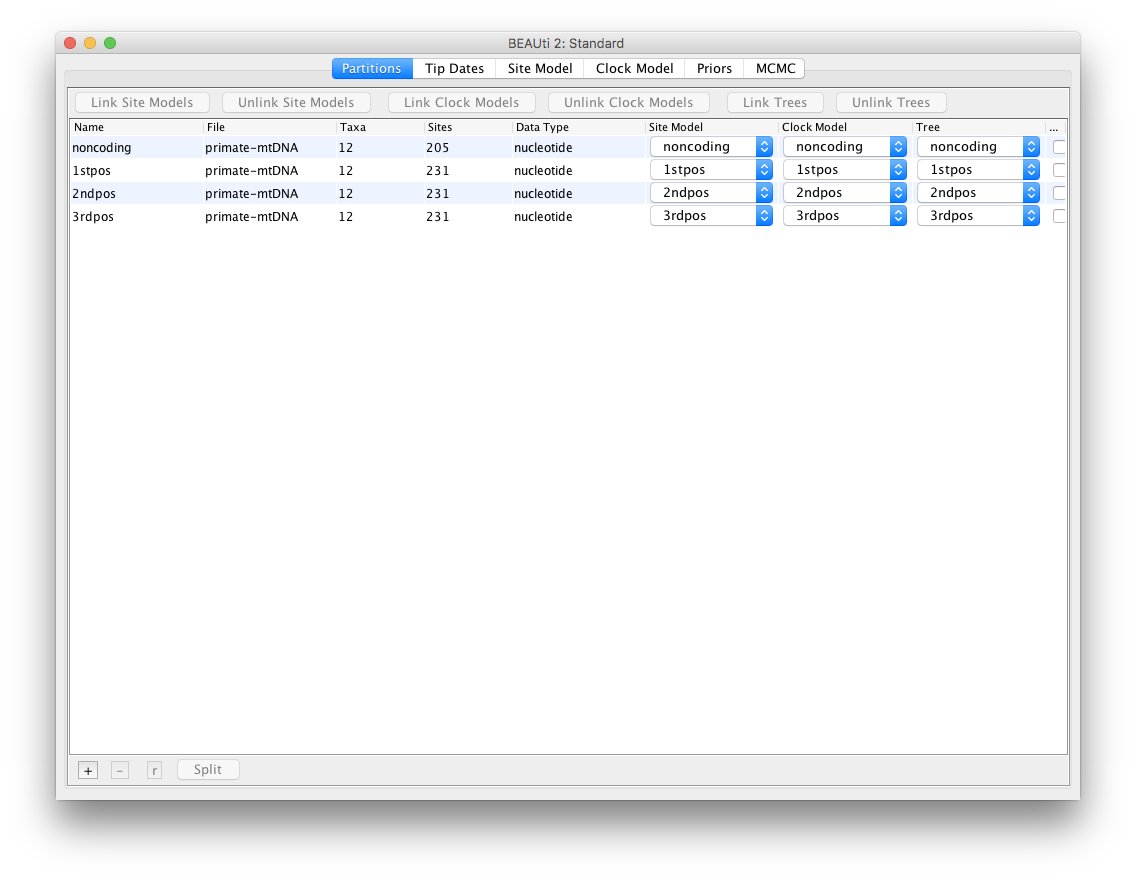
\includegraphics[width=5in]{figures/data.png}
\caption{\small Data imported into BEAUti}
\label{fig:data}
\end{figure}

\subsubsection{Setting up shared models}

One way to account for variation in substitution rates between different sites is to include gamma rate categories. In this scenario, one defines a Gamma distribution and discretises it in the desired number of bins (4-6 usually). The mean of each bin is then acting as a multiplier for the overall substitution rate. The transitions probabilities are then calculated for each scaled substitution rate. P(data | tree, substitution model) can then be calculated under each gamma rate category and the results are summed up to average over all possible rates. This is a handy approach if one suspects that some sites can be mutating faster than others but the precise position of the sites in the alignment is unknown or random.

Another way to account for site rate heterogeneity is to split the alignment into explicit partitions. This is especially relevant, when one knows exactly which positions in the alignment have different substitution rates from the rest of the sites. In our example, we split the alignment into coding and non-coding parts, and split the coding part further into 1st, 2nd and 3rd codon positions. We can now specify a separate substitution model for each partition. 

Since all of the sequences in this data set are from the mitochondrial genome (which is not believed to undergo recombination in birds and mammals) they all share the same ancestry. By default BEAST2 would recover a time-tree for each partition, so we need to make sure that it uses all data to recover a single shared tree. For the sake of simplicity, we will also assume the partitions have the same evolutionary rate for each branch, and hence share the clock model as well.

To make sure that the partitions share the same evolutionary history we need to link the clock model and the tree in BEAUti, which can be done by selecting all four partitions and clicking the \texttt{Link Trees} and {Link Clock Models} buttons.

\begin{framed}
Select all four data partitions the \texttt{Partitions} panel and click the \texttt{Link Trees} and {Link Clock Models} buttons.
\end{framed}

You will see that the \texttt{Clock Model} and the \texttt{Tree} columns in the table both changed to say \texttt{noncoding}. Now we will rename both models such that the following options and generated log files more easy to read. The resulting setup should look as shown in Figure~\ref{fig:link}.

\begin{framed}
Click on the first drop-down menu in the \texttt{Clock Model} column and rename the shared clock model to \texttt{clock}.

Likewise rename the shared tree to \texttt{tree}.
\end{framed}

\begin{figure}[!h]
\centering
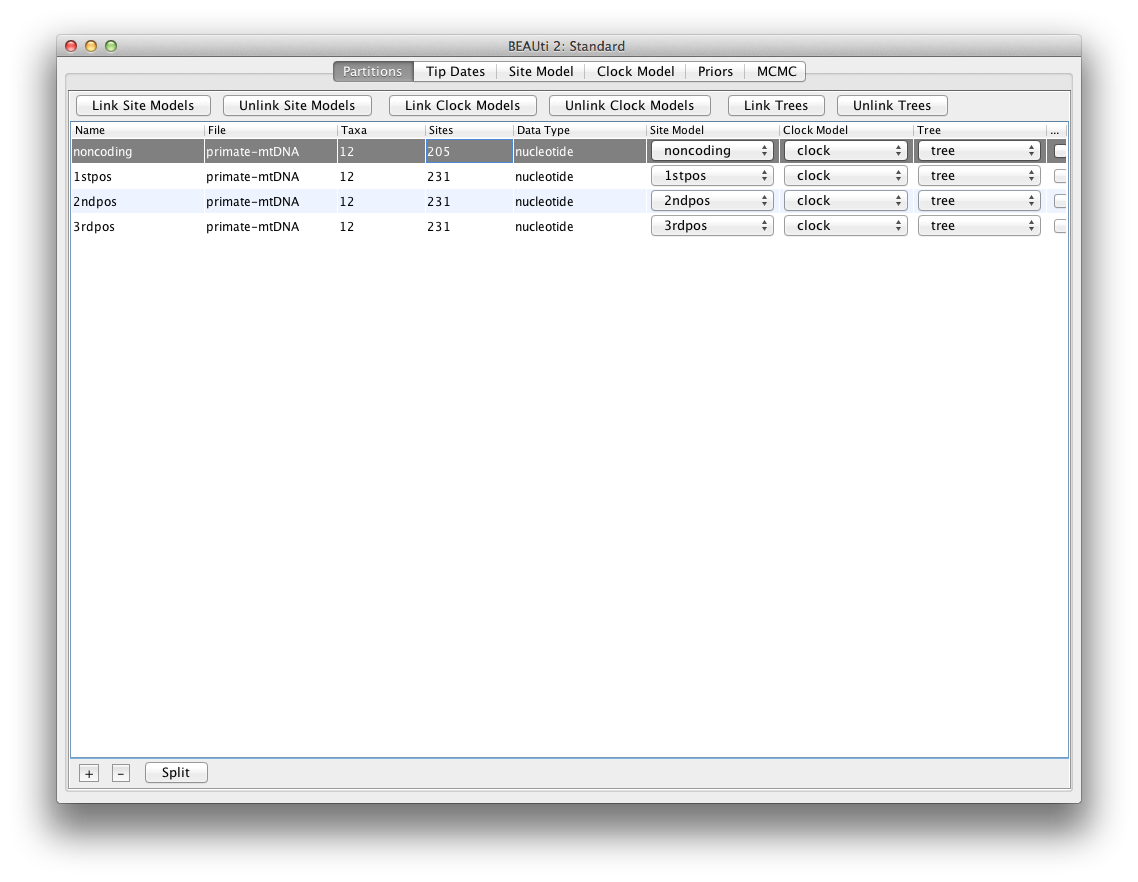
\includegraphics[width=5in]{figures/link.png}
\caption{\small Linked models}
\label{fig:link}
\end{figure}

\subsubsection{Setting the substitution model}

Next we need to set up the substitution model in the \texttt{Site Model} tab.

\begin{framed}
Select the \texttt{Site Model} tab.
\end{framed}

The options available in this panel depend on whether the alignment data is in nucleotides, aminoacids, binary data or general data. The settings available after loading the alignment will contain the default values which we normally want to modify.

The panel on the left shows each part of the alignment. Remember that we did not link the substitution models in the previous step for the different partition, so each partition is allowed to evolve under different substitution model, i.e. we assume that different positions in the alignment accumulate substitutions differently. We will need to set the site substitution model separately for each part of the alignment as these models are unlinked. However, we think that all partitions evolve according to the same model (although with different parameters) so we can temporarily link the site models in the \texttt{Partitions} panel so that we can change the model of all partitions simultaneously. 

Navigate to the \texttt{Partitions} tab again, select all the partitions and temporarily link the site models. Then go back to the \texttt{Site Model} tab. The panel on the left is now gone as we are setting one model for all of the partitions.

\begin{framed}
Go to the \texttt{Partitions} tab, select all partitions and click the \texttt{Link Site Models} button.

Return to the \texttt{Site Model} tab.
\end{framed}

First, check the \texttt{estimate} checkbox at the \texttt{Substitution Rate}, as we want to estimate relative substitution rates for each partition. Next, set the \texttt{Gamma Category Count} to 4 and check the \texttt{estimate} box for the \texttt{Shape} parameter. This will allow rate variation between sites in each partition to be modelled. Then select \texttt{HKY} in the \texttt{Subst Model} drop-down and select \texttt{Empirical} from the \texttt{Frequencies} drop-down. This will fix the frequencies to the proportions observed in the data (for each partition individually, once we unlink the site models again). This approach means that we can get a good fit to the data without explicitly estimating these parameters. The setup should look now as shown in Figure~\ref{fig:subst}.

\begin{framed}
Check the \texttt{estimate} checkbox at the \texttt{Substitution Rate}.

Set the \texttt{Gamma Category Count} to 4.

Check the \texttt{estimate} box for the \texttt{Shape} parameter.

Select \texttt{HKY} in the \texttt{Subst Model} drop-down.

Select \texttt{Empirical} from the \texttt{Frequencies} drop-down.
\end{framed}

Now return to the \texttt{Partitions} panel and unlink the site models such that each partition has its own named site model with independent substitution model parameters and relative rate. You can make sure this is the case by returning to the \texttt{Site Model} tab and clicking through the different partitions. 

\begin{framed}
Go to the \texttt{Partitions} tab again, select all partitions and click the \texttt{Unlink Site Models} button.
\end{framed}

\begin{figure}[!h]
\centering
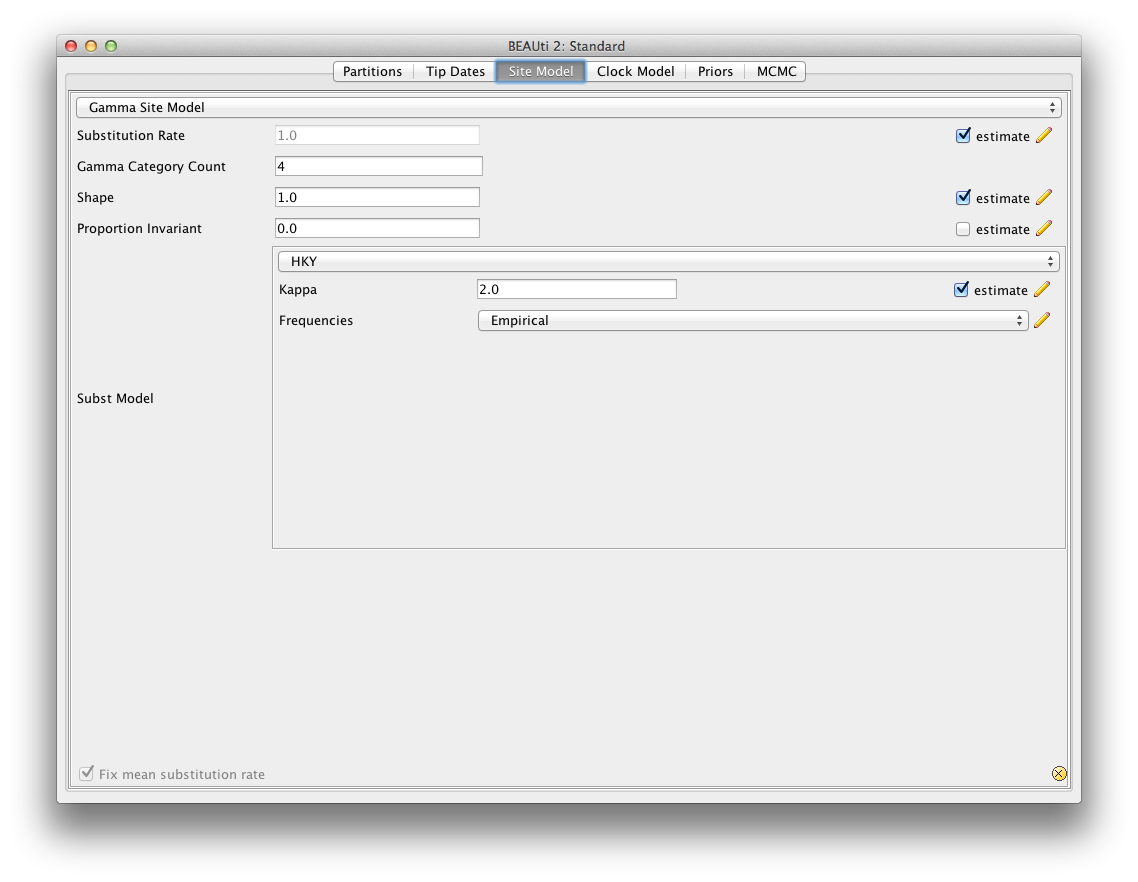
\includegraphics[width=5in]{figures/substitution.png}
\caption{\small Substitution model setup}
\label{fig:subst}
\end{figure}

\subsubsection{Setting the clock model}

Next, select the \texttt{Clock Models} tab at the top of the main window. This is where we set up the molecular clock model. For this exercise we are going to leave the selection at the default value of a strict molecular clock, because this data is very clock-like and does not need rate variation among branches to be included in the model.

\begin{framed}
Go to the \texttt{Clock Models} tab and view the setup.
\end{framed}

\subsubsection{Setting priors}

The \texttt{Priors} tab allows priors to be specified for each parameter in the model. The model selections made in the site model and clock model tabs, result in the inclusion of various parameters in the model. For each of these parameters a prior distribution needs to be specified.

Here we specify that we wish to use the Calibrated Yule model as the tree prior. This is a simple model of speciation that is generally more appropriate when considering sequences from different species.

\begin{framed}
Go to the \texttt{Priors} tab and select the \texttt{Calibrated Yule Model} in the \texttt{Tree.t:tree} dropdown menu.
\end{framed}

We will set the prior for \texttt{birthRateY.t:tree} to a \texttt{Gamma} distribution with an \texttt{Alpha} of 0.001 and \texttt{Beta} of 1000.

\begin{framed}
For \texttt{birthRateY.t:tree} select \texttt{Gamma} from the dropdown menu,

Expand the options for \texttt{birthRateY.t:tree} using the arrow button on the left.

Set the \texttt{Alpha} (shape) parameter to 0.001 and the \texttt{Beta} (scale) parameter to 1000.
\end{framed}

We will leave the rest of the priors on their default values, which should look as shown in Figure~\ref{fig:priors}.

Please note that in general using default priors is highly frowned upon as priors are meant to convey your prior knowledge of the parameters. It is important to know what exactly do the priors tell MCMC and whether this fits your particular situation. In our case the default priors are suitable for this particular analysis, however for further, more complex analyses, we will require a clear idea of what do the priors mean. Getting this understanding is hard so we will leave it to the later Taming the Beast classes and tutorials in order to keep the introduction as simple as possible.

\begin{figure}[!h]
\centering
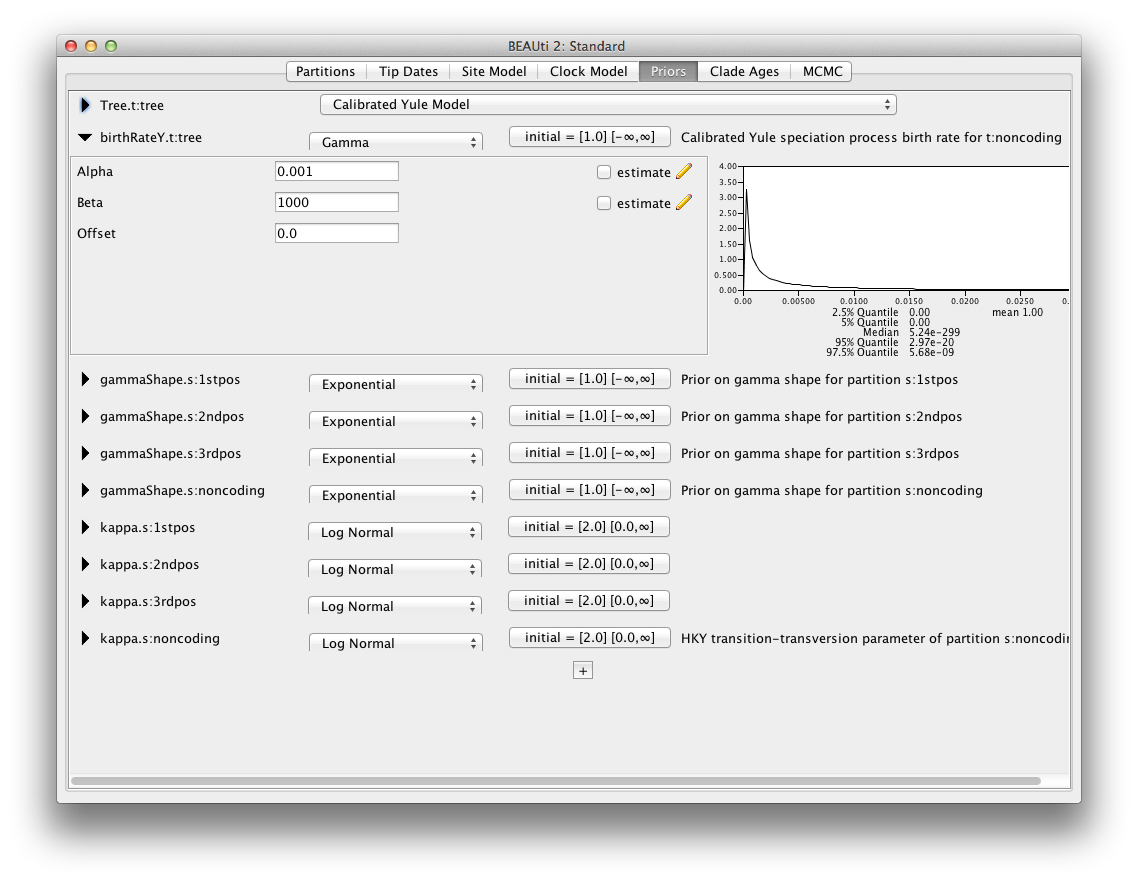
\includegraphics[width=5in]{figures/priors.png}
\caption{\small Prior setup}
\label{fig:priors}
\end{figure}

\subsubsection{Adding a calibration node}

Since all of the samples come from a single time point, there is no information on the actual height of the phylogenetic tree in time units. Tree height and substitution rate will not be distinguishable and BEAST2 will only be able to estimate their product. To give BEAST2 the possibility to separate these two parameters we need to input additional information that will help calibrate the tree in time.

Since in the Bayesian analysis such information should be encoded in the form of a prior distribution, we will have to add a new prior that is not available yet. To define an extra prior, press the small \texttt{+} button below list of priors. You will see a dialogue that allows you to define a subset of the taxa in the phylogenetic tree. Once you have created a taxa set you will be able to add calibration information for its most recent common ancestor (MRCA) later on.

\begin{framed}
Click the small \texttt{+} button below all the priors.
\end{framed}

Name the taxa set by filling in the taxon set label entry. Call it human-chimp (it will contain the taxa for Homo sapiens and Pan). In next list below you will see the available taxa. Select and add the Homo sapiens and Pan taxa to the set (see Figure~\ref{fig:taxa}). After you click \texttt{OK} and the newly defined taxa set will be added to the prior list.

\begin{framed}
Set the \texttt{Taxon set label} to \texttt{human-chimp}.

Locate \texttt{Homo\_sapiens} taxon in the left hand side list and click the \texttt{>>} button to add it to the taxa set for \texttt{human-chimp}.

Locate \texttt{Pan} taxon in the left hand side list and click the \texttt{>>} button to add it to the taxa set for \texttt{human-chimp}.

Click the \texttt{OK} button to add the newly defined taxa set to the prior list.
\end{framed}

\begin{figure}[!h]
\centering
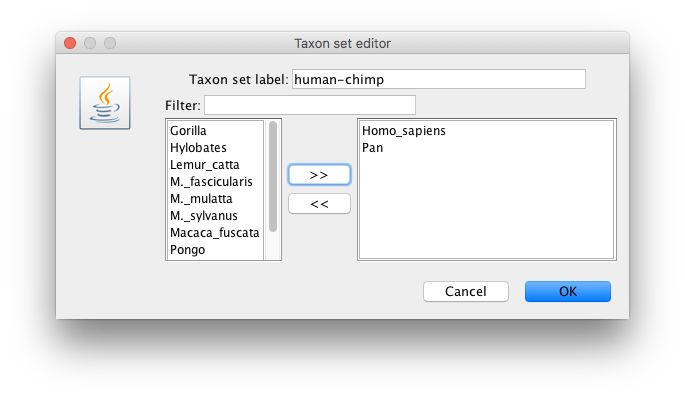
\includegraphics[width=5in]{figures/taxa.png}
\caption{\small Calibration node taxa set definition}
\label{fig:taxa}
\end{figure}

The new node we have added is a calibrated node to be used in conjunction with the Calibrated Yule prior. In order for that to work we need to enforce monophyly, so select the checkbox marked Monophyletic. This will constrain the tree topology so that the human-chimp grouping is kept monophyletic during the course of the MCMC analysis.

\begin{framed}
Check the \texttt{monophyletic} checkbox next to the \texttt{human-chimp.prior}.
\end{framed}

We now need to specify a prior distribution on the calibration node based on our prior fossil knowledge in order to calibrate our tree. Select the \texttt{Normal} distribution for the newly added \texttt{human-chimp.prior}. Expand the prior options and  specify a normal distribution centred at 6 million years with a standard deviation of 0.5 million years. This will give a central 95\% range of about 5-7 million years. This roughly corresponds to the current consensus estimate of the date of the most recent common ancestor of humans and chimpanzees.

\begin{framed}
Select the \texttt{Normal} distribution from the drop down menu to the right of the newly added \texttt{human-chimp.prior}.

Expand the distribution options using the arrow button on the left.

Set the \texttt{Mean} of the distribution to 6.

Set the \texttt{Sigma} of the distribution to 0.5.
\end{framed}

The final setup of the calibration node should look as shown in Figure~\ref{fig:calibration}.

\begin{figure}[!h]
\centering
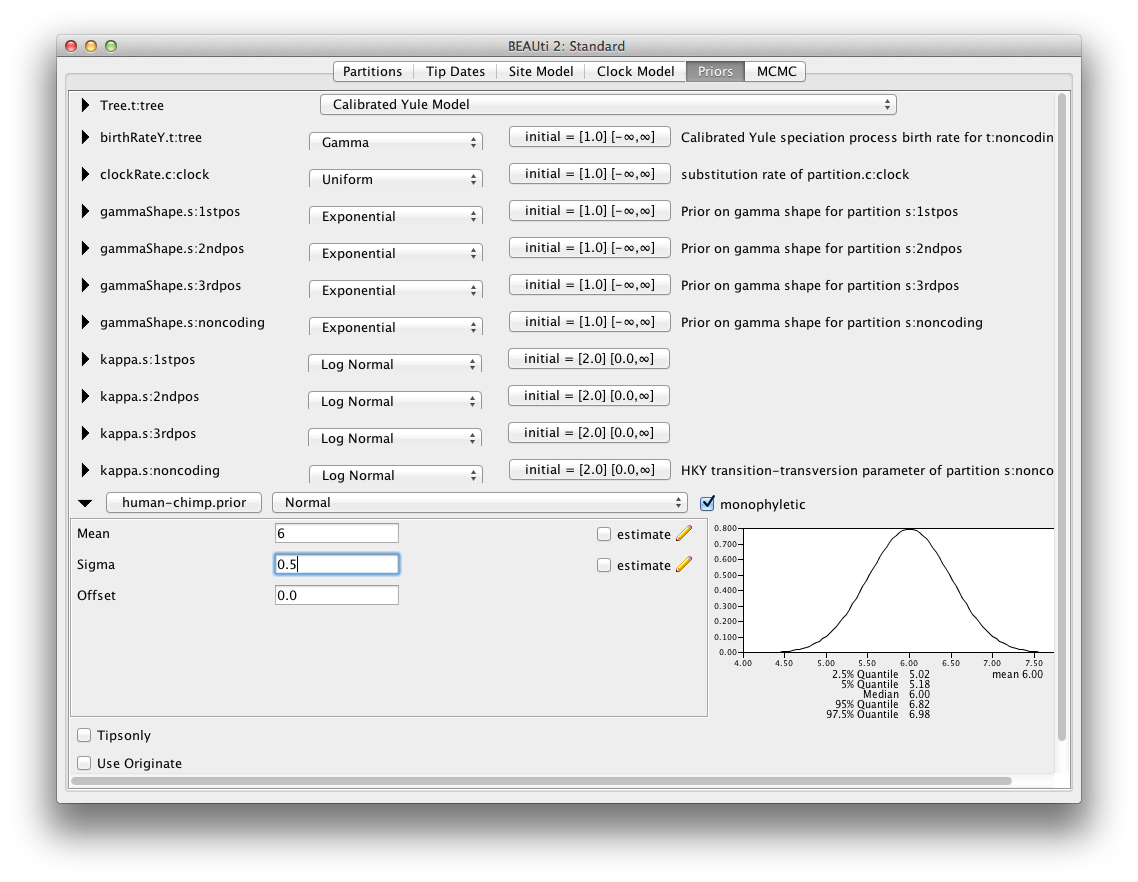
\includegraphics[width=5in]{figures/calibration.png}
\caption{\small Calibration node prior setup}
\label{fig:calibration}
\end{figure}

\subsubsection{Setting the MCMC options}

Finally, the \texttt{MCMC} tab allows to control the length of the MCMC run and frequency of stored samples. It also allows one to change the output file names.

\begin{framed}
Go to the \texttt{MCMC} tab.
\end{framed}

The \texttt{Chain Length} parameter specifies the number of steps the MCMC chain will make before finishing. This number depends on the size of the dataset, the complexity of the model and the precision of the answer required. The default value of 10'000'000 is arbitrary and should be adjusted accordingly. For this small dataset we initially set the chain length to 1'000'000 such that this analysis will take only a few minutes on most modern computers (rather than hours). For now we leave the \texttt{Store Every} and \texttt{Pre Burnin} fields at their default values.

\begin{framed}
Set the \texttt{Chain Length} to 1'000'000.
\end{framed}

Below these general settings you will find the logging settings. Each particular logging option can be viewed in detail by clicking the arrow to the left of it. You can control the names of the log files and how often should the values be stored in each of the files.

Start by expanding the \texttt{tracelog} options. This is the log file you will use later to analyse and summarise the results of the run. The \texttt{Log Every} parameter for the log file should be set relative to the total length of the chain. Sampling too often will result in very large files with little extra benefit in terms of the accuracy of the analysis. Sampling too rarely will mean that the log file will not record sufficient information about the distributions of the parameters. We normally want to aim to store no more than 10'000 samples so this should be set to no less than chain length/10'000. For this analysis we will make BEAST2 write to log file every 200 samples.

\begin{framed}
Expand the \texttt{tracelog} options.

Set the \texttt{Log Every} parameter to 200.
\end{framed}

Then, expand the \texttt{screenlog} options. The screen output is simply for monitoring the program's progress. Since it is not so important, especially if you run your analysis on a remote computer or a computer cluster, the \texttt{Log Every} can be set to any value. Although if set too small, the sheer quantity of information being displayed on the screen will actually slow the program down. For this analysis we will make BEAST2 log to screen every 1'000 samples, which is the default setting.

\begin{framed}
Expand the \texttt{screenlog} options.

Leave the \texttt{Log Every} parameter at the default value of 1'000.
\end{framed}

Finally, we can also change the tree logging frequency by expanding the \texttt{treelog.t:tree}. Set the sampling frequency to 1'000 and rename the tree log file to \texttt{primate-mtDNA.trees}.

\begin{framed}
Expand the \texttt{treelog.t:tree} options.

Set the \texttt{File Name} to \texttt{primate-mtDNA.trees}.

Leave the \texttt{Log Every} parameter at the default value of 1'000.
\end{framed}

The final setup should look as in Figure~\ref{fig:logs}.

\begin{figure}[!h]
\centering
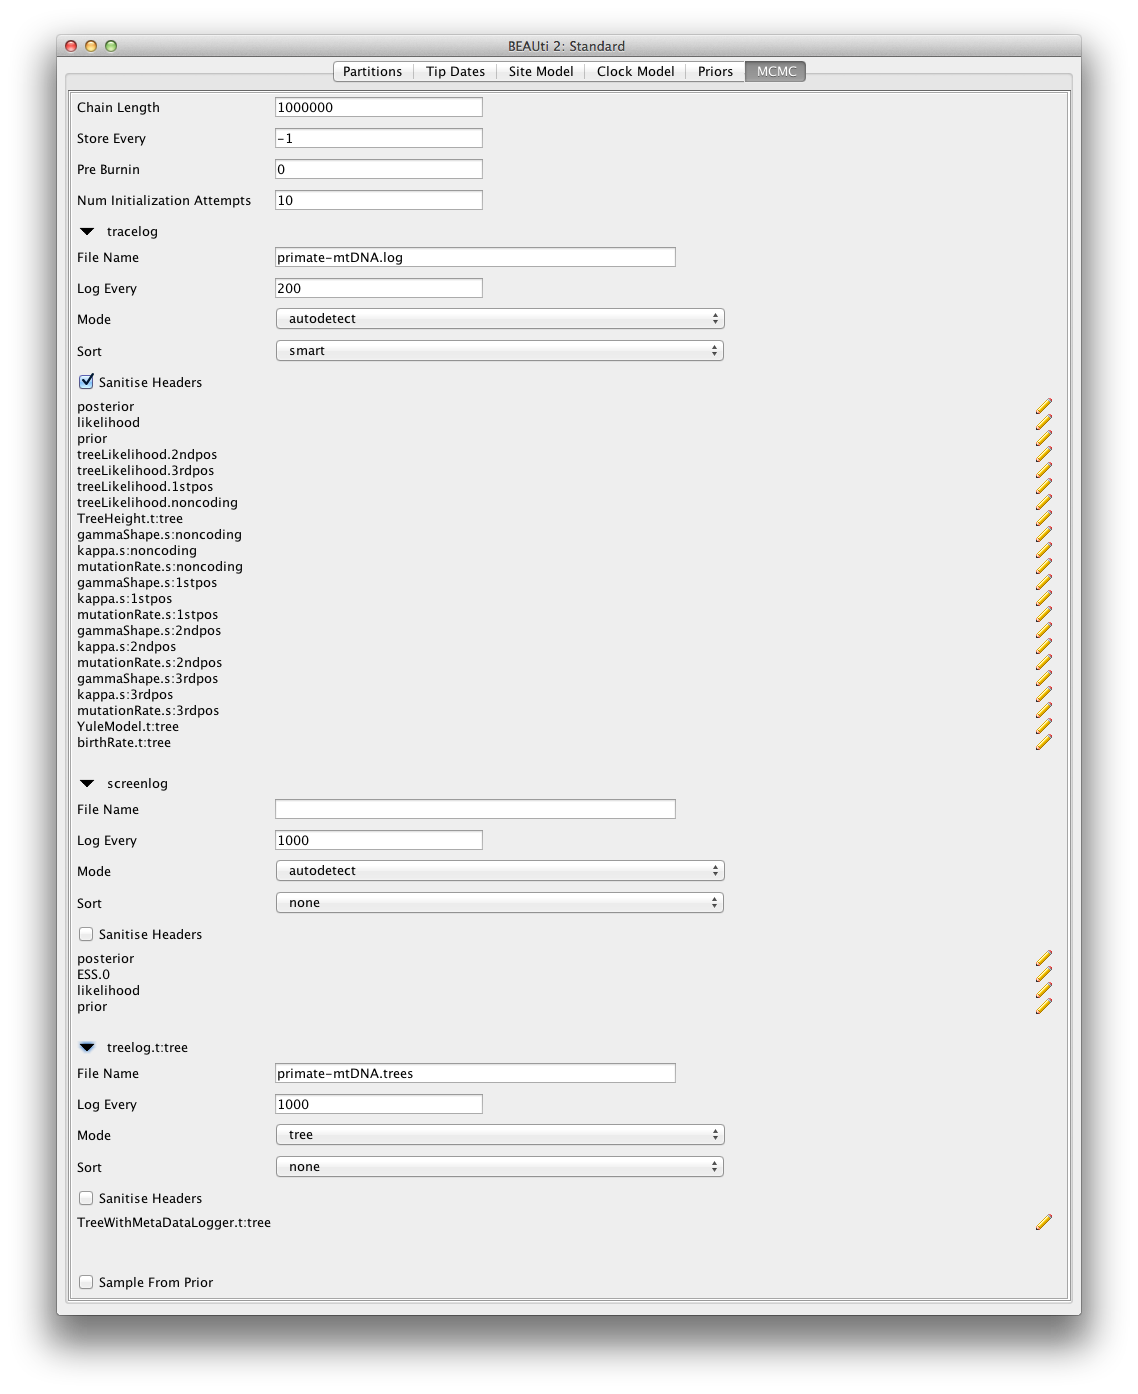
\includegraphics[width=5in]{figures/logs.png}
\caption{\small Logging options}
\label{fig:logs}
\end{figure}

\subsubsection{Generating the XML file}

We are now ready to create the BEAST2 XML file. To do this, select \texttt{File > Save}, and save the file with an appropriate name (we usually end the filename with .xml, i.e. Primates.xml). This is the final configuration file BEAST2 can use to execute the analysis.

\begin{framed}
Save the XML file under the name Primates.xml using \texttt{File > Save}.
\end{framed}

\subsection{Running the analysis}

Now run BEAST2 and provide your newly created XML file as input. You can also change the \texttt{Random number seed} for the run. This number is the starting point of a pseudo-random number chain BEAST2 will use to generate the samples. As computers are unable to generate truly random numbers, we have to resort to generating determinate sequences of numbers that only look random, but will be identical when the starting seed is the same.

\begin{framed}
Run the BEAST2 program.

Select Primates.xml as the \texttt{Beast XML File}.
\end{framed}

For this run we will set the \texttt{Random number seed} to 777 (or any other number you like). The BEAST2 window should look as shown in Figure~\ref{fig:beast}. 

\begin{framed}
Set the \texttt{Random number seed} to 777 (or pick your favourite number).
\end{framed}

Now you can run the analysis by pressing the \texttt{Run} button at the bottom of the window. BEAST2 will run until the specified number of steps in the chain is reached. While it is running, it will print the screenlog values to a console and store the tracelog and tree log values to files located in the same folder as the configuration XML file. The screen output will look approximately as shown in Figure~\ref{fig:beast_out}.

\begin{framed}
Run BEAST2 by clicking the \texttt{Run} button.
\end{framed}

The window will remain open when BEAST2 will finished. When you try to close it, you may see BEAST2 asking the question: "Do you wish to save?". Note that your log and trees files are always saved, no matter what answer you choose for this question. Thus, the question is only restricted to saving or not of the BEAST2 \texttt{screenlog} output. In order to save this output, click \texttt{Yes} and select the location on your computer, and the filename under which you wish to save this output. However, for now, it is safe to click \texttt{No} and not save the \texttt{screenlog} output.

\begin{figure}[!h]
\centering
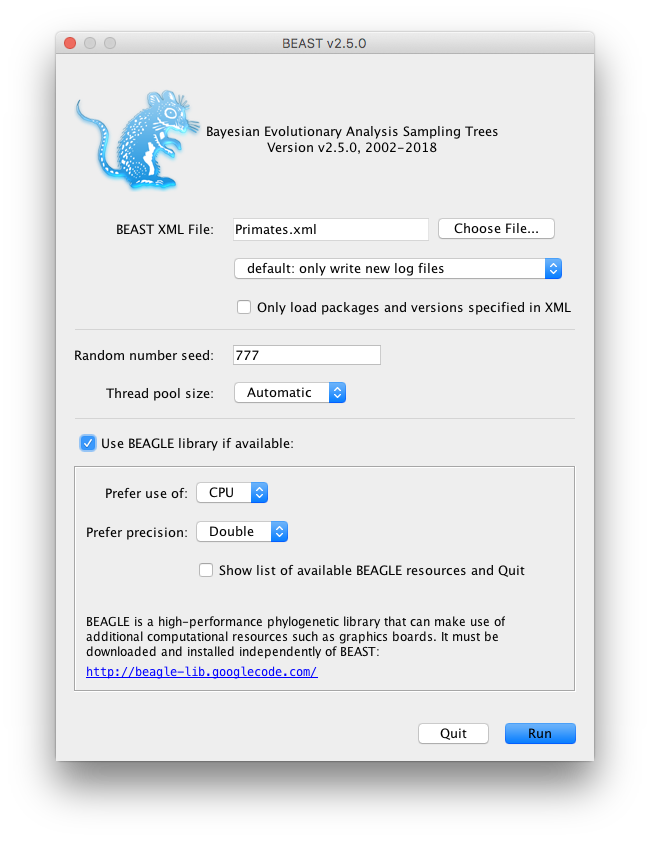
\includegraphics[width=5in]{figures/beast.png}
\caption{\small BEAST2 setup for the analysis}
\label{fig:beast}
\end{figure}

\begin{figure}[!h]
\centering
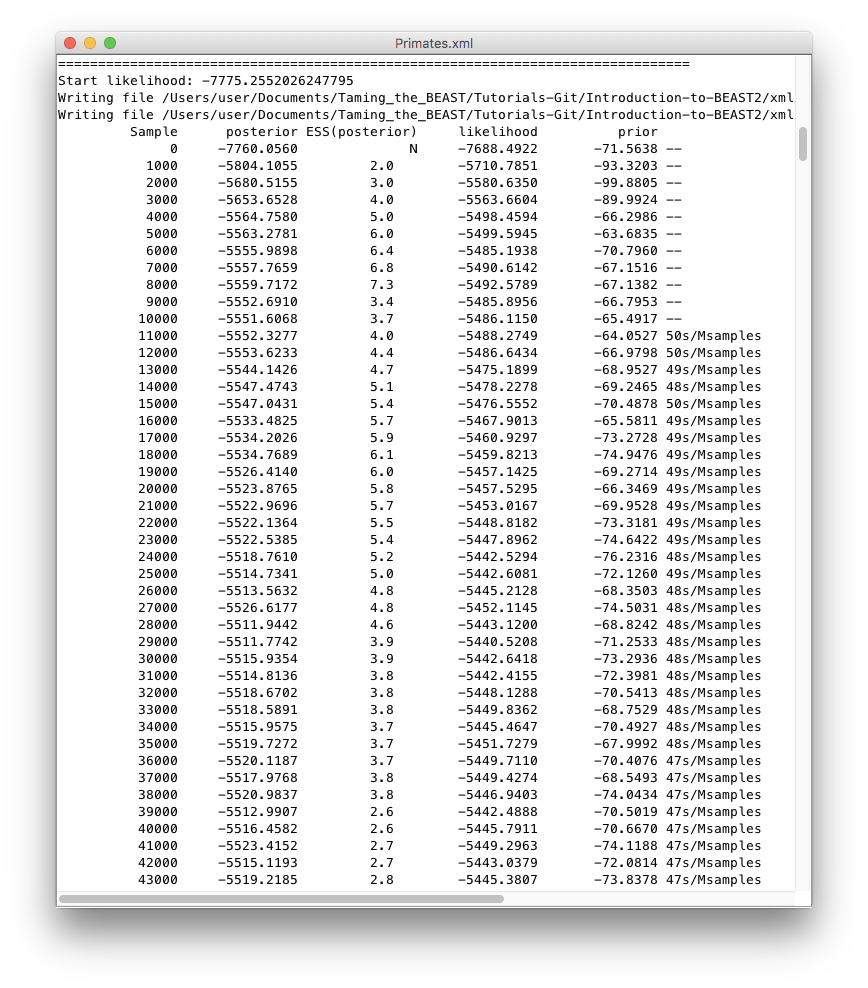
\includegraphics[width=5in]{figures/beast_out.png}
\caption{\small BEAST2 output for the analysis}
\label{fig:beast_out}
\end{figure}

\subsection{Analysing parameter estimates}

Once BEAST2 has finished running, open Tracer to get an overview of BEAST2 output. When the main window has opened, choose \texttt{File > Import Trace File...} and select the file called \texttt{primate-mtDNA.log} that BEAST2 has created, or simply drag the file from the file manager window into Tracer. The Tracer window should look as shown in Figure~\ref{fig:tracer_bad}.

\begin{framed}
Open Tracer.

Use \texttt{File > Import Trace File...} to load the \texttt{primate-mtDNA.log} file that BEAST2 has created.
\end{framed}

Tracer provides a few useful summary statistics on the results of the analysis. On the left side in the top window it provides a list of log files loaded into the program at the moment. The window below shows the list of statistics logged in each file. For each statistic it gives a list of summary values such as the mean, standard error, median, and others it can compute from the data. The summary values are displayed in the top right window and the distribution of the statistic is shown in the graphics in the bottom right window. 

The log file contains traces for the posterior (this is the natural logarithm of the product of the tree likelihood and the prior density), prior, the likelihood, the tree likelihood and the continuous parameters. Selecting a trace on the left brings up the summary statistics for this trace on the right hand side. When first opened, the \texttt{posterior} trace is selected and various statistics of this trace are shown under the \texttt{Estimates} tab.

For each loaded log file we can specify a \texttt{Burn-In}, which is shown in the file list table (top-left) in Tracer. The burn-in is intended to give the Markov Chain time to reach its equilibrium distribution, particularly if it has started from a bad starting point. A bad starting point may lead to over-sampling regions of the posterior that actually have very low probability under the equilibrium distribution, before the chain settles into the equilibrium distribution. Burn-in allows us to simply discard the first N samples of a chain and not use them to compute the summary statistics. Determining the right number of samples to throw out is more of an art form than a technique (as we cannot predict when the chain will reach equilibrium), so we normally simply settle for specifying first 10\% of the whole chain length as the burn-in.

Select the \texttt{TreeHeight} statistic in the left hand list to look at the tree height estimated jointly for all of the partitions in the alignment. Tracer will plot a (marginal posterior) histogram for the selected statistic and also give you summary statistics such as the mean and median. The 95\% HPD stands for \textit{highest posterior density interval} and represents the most compact interval on the selected statistic that contains 95\% of the posterior probability. It can be loosely thought of as a Bayesian analogue to a confidence interval. The \texttt{TreeHeight} statistic gives the marginal posterior distribution of the age of the root of the entire tree.

\begin{framed}
Select the \texttt{TreeHeight} statistic in the bottom left hand list in Tracer and view the different summary statistics on the right.
\end{framed}

You can also compare estimates of different parameters in Tracer. Once a trace file is loaded into the program you can, for example, compare estimates of the different mutation rates corresponding to different positions in the alignment. Select all four mutation rate traces and then select the \texttt{Marginal Prob Distribution} tab on the right. You will be able to see all four distributions in one plot, similar to what is shown in Figure~\ref{fig:tracer_comparison}.

\begin{framed}
Select all four mutation rates by clicking the first mutation rate (\texttt{mutationRate.noncoding}), then holding \texttt{Shift} and clicking the last mutation rate (\texttt{mutationRate.3rdpos}).

Select the \texttt{Marginal Prob Distribution} tab on the right to view the four distributions together.
\end{framed}

\begin{figure}[!h]
\centering
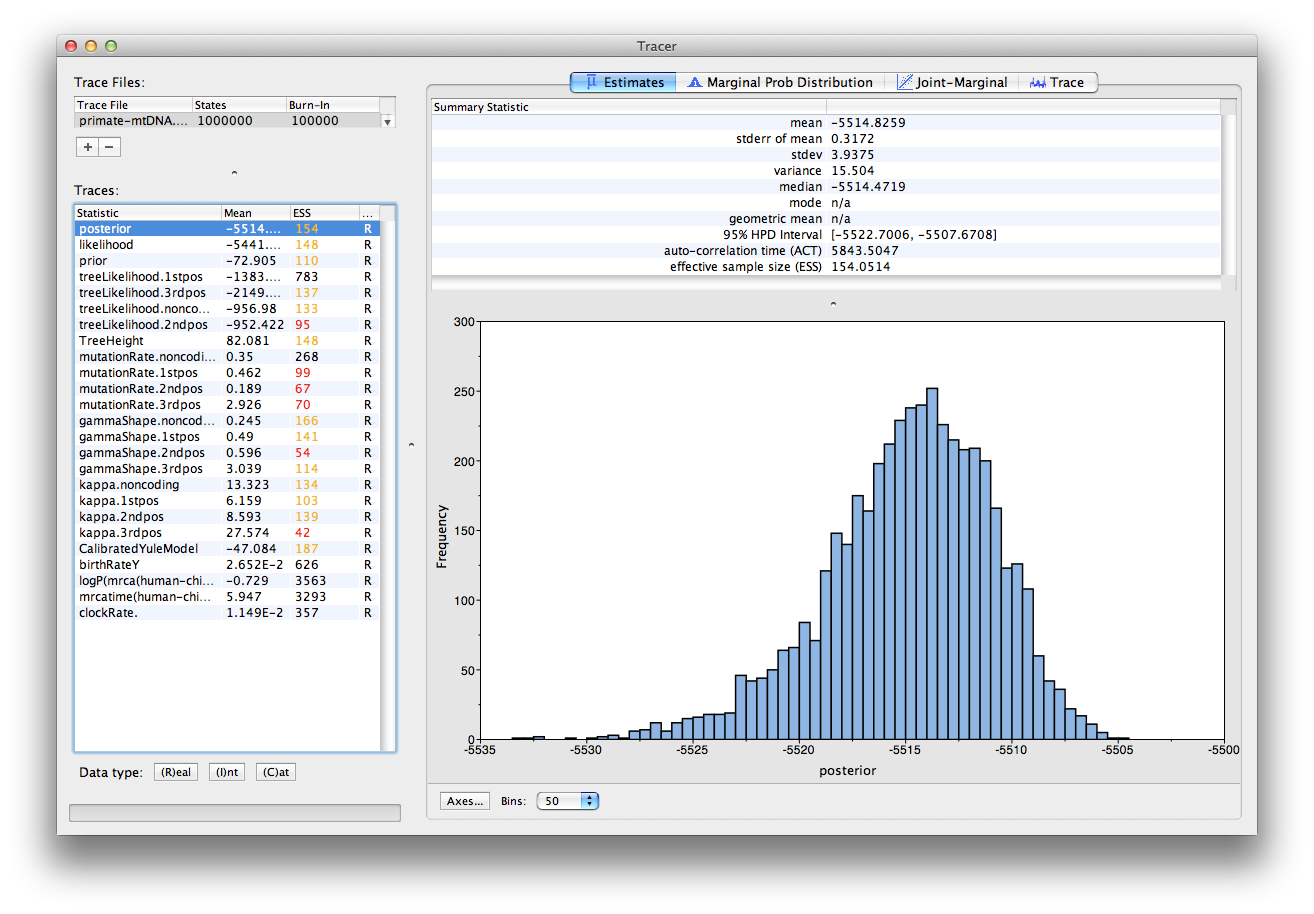
\includegraphics[width=5in]{figures/tracer_bad.png}
\caption{\small Tracer showing a summary of the BEAST2 run of primate data with MCMC chain length of 1'000'000.}
\label{fig:tracer_bad}
\end{figure}

\begin{figure}[!h]
\centering
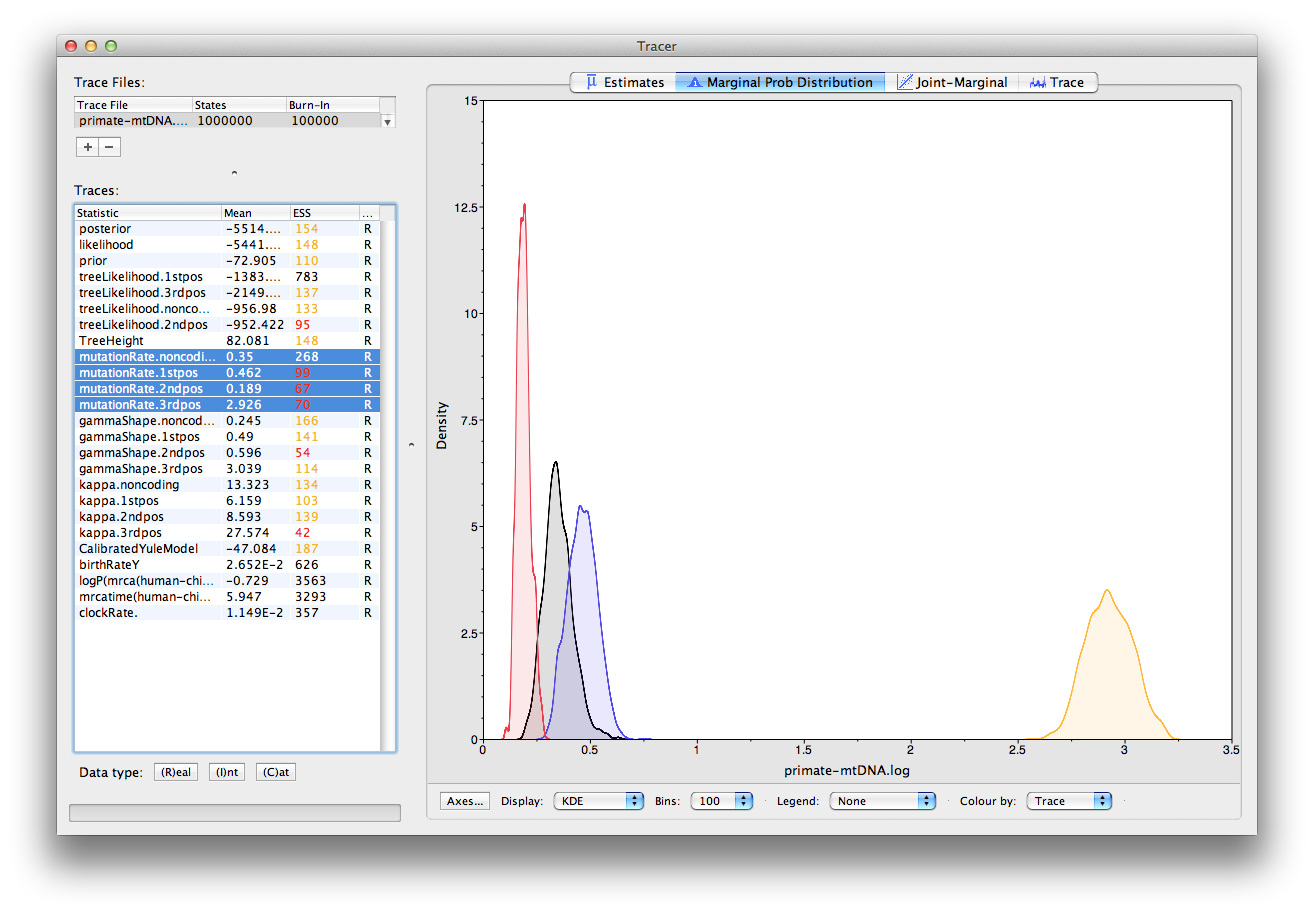
\includegraphics[width=5in]{figures/tracer_comparison.png}
\caption{\small Tracer showing the four marginal probability distributions of the mutation rates in each partition of the alignment.}
\label{fig:tracer_comparison}
\end{figure}

\subsubsection{Analysing the posterior estimate quality}

Two very important summary statistics that we should pay attention to are the Auto-Correlation Time (ACT) and the Effective Sample Size (ESS). ACT is the average number of states in the MCMC chain that two samples have to be separated by for them to be uncorrelated, i.e. for them to be independent samples from the posterior. The ACT is estimated from the samples in the trace (excluding the burn-in). The ESS is the number of independent samples that the trace is equivalent to. This is calculated as the chain length (excluding the burn-in) divided by the ACT.

The ESS is in general regarded as a quality-measure of the resulting sample sequence. It is unclear how to determine exactly how large should the ESS be for the analysis to be trustworthy so an empirical number was defined. In general, an ESS of 200 will be considered enough to make the analysis useful. As you can see in Figure~\ref{fig:tracer_bad}, ESS values below 100 are coloured in red, which means that we should not trust the value of the statistics, and ESS values between 100 and 200 are coloured in yellow.

If a lot of statistics have red or yellow coloured ESS value, we did not explore the posterior space sufficiently. This is most likely a result of the chain not running long enough. Try running the same analysis, but first load the XML configuration file into BEAUti again by pressing \texttt{File > Load} and select the Primates.xml file.  Within BEAUti, change the MCMC chain length parameter to 2'500'000. Change the trace and tree log file names in order for not over-writing the results of the previous analysis. You may add something like \texttt{\_long} behind the name of the file, to obtain \texttt{primate-mtDNA\_long.log} for the log file and \texttt{primate-mtDNA\_long.trees} for trees file. Run BEAST2 again with the updated configuration and the seed of 777. This will take a bit more time. Figure~\ref{fig:tracer_better} shows the estimates from a longer run. The ESS of 200 is still not reached for the \texttt{TreeHeight} parameter (and few other parameter), but it did turn higher than the ESS obtained with the shorter chain. This means that if we allow the chain to run even longer we will most likely reach good ESS values for this parameter as well.

Remember that MCMC is a stochastic algorithm, so if you set a different seed the actual numbers will not be exactly the same as those depicted in the figure.% However, if you run the analysis twice with the same seed, but with a longer chain the second time, the second trace will include the first one, as the start of the random number sequence will be the same. To verify that, select both trace files in Tracer, pick any statistic and select the \texttt{Trace} tab on the right. Figure~\ref{fig:tracer_two} shows what it should look like when we tell Tracer to colour traces by trace file (pick \texttt{Trace file} in the \texttt{Colour by} drop down menu at the very bottom of the window).

\begin{figure}[!h]
\centering
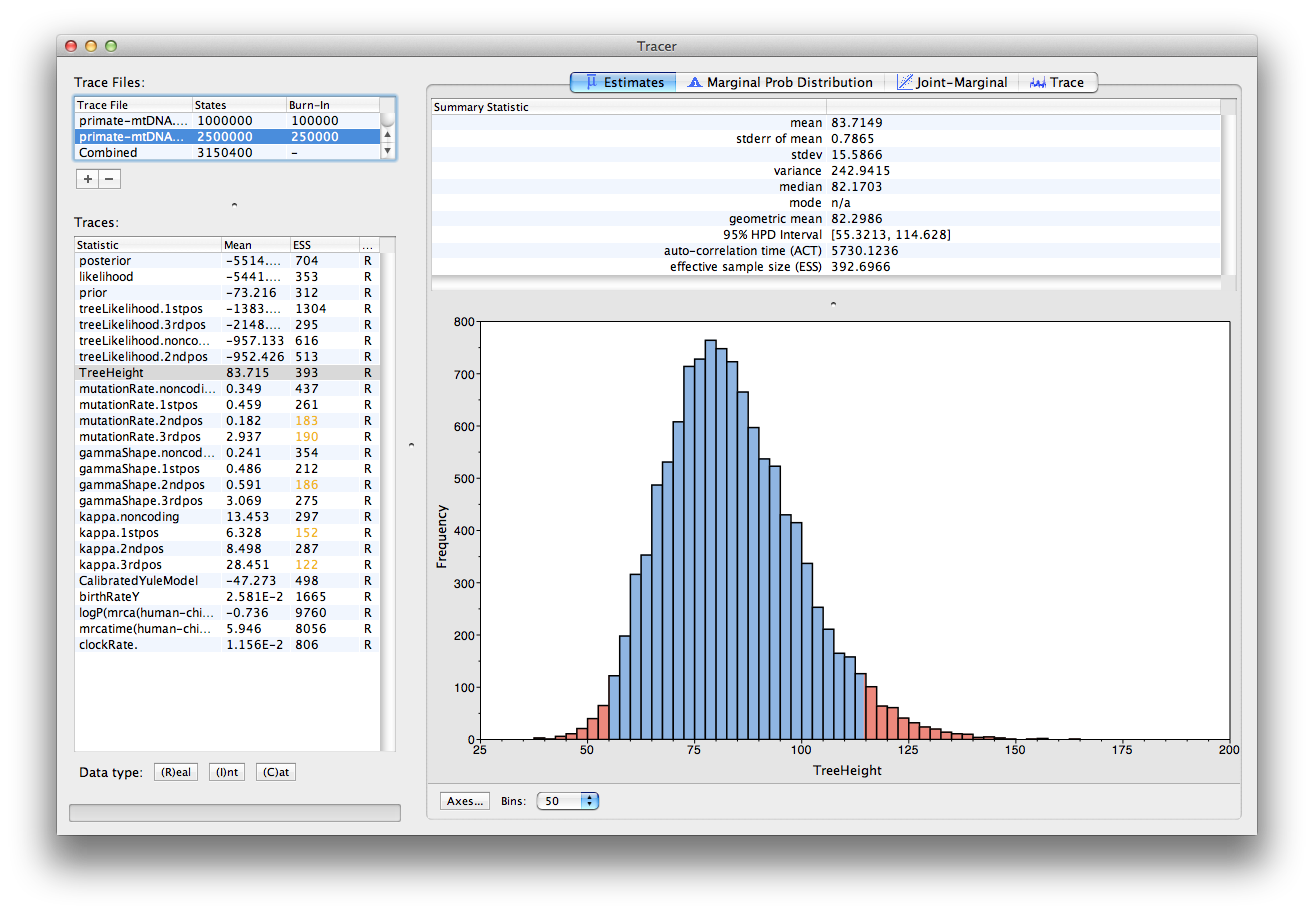
\includegraphics[width=5in]{figures/tracer_better.png}
\caption{\small Tracer showing a summary of the BEAST2 run with MCMC chain length of 2'500'000.}
\label{fig:tracer_better}
\end{figure}

%\begin{figure}[!h]
%\centering
%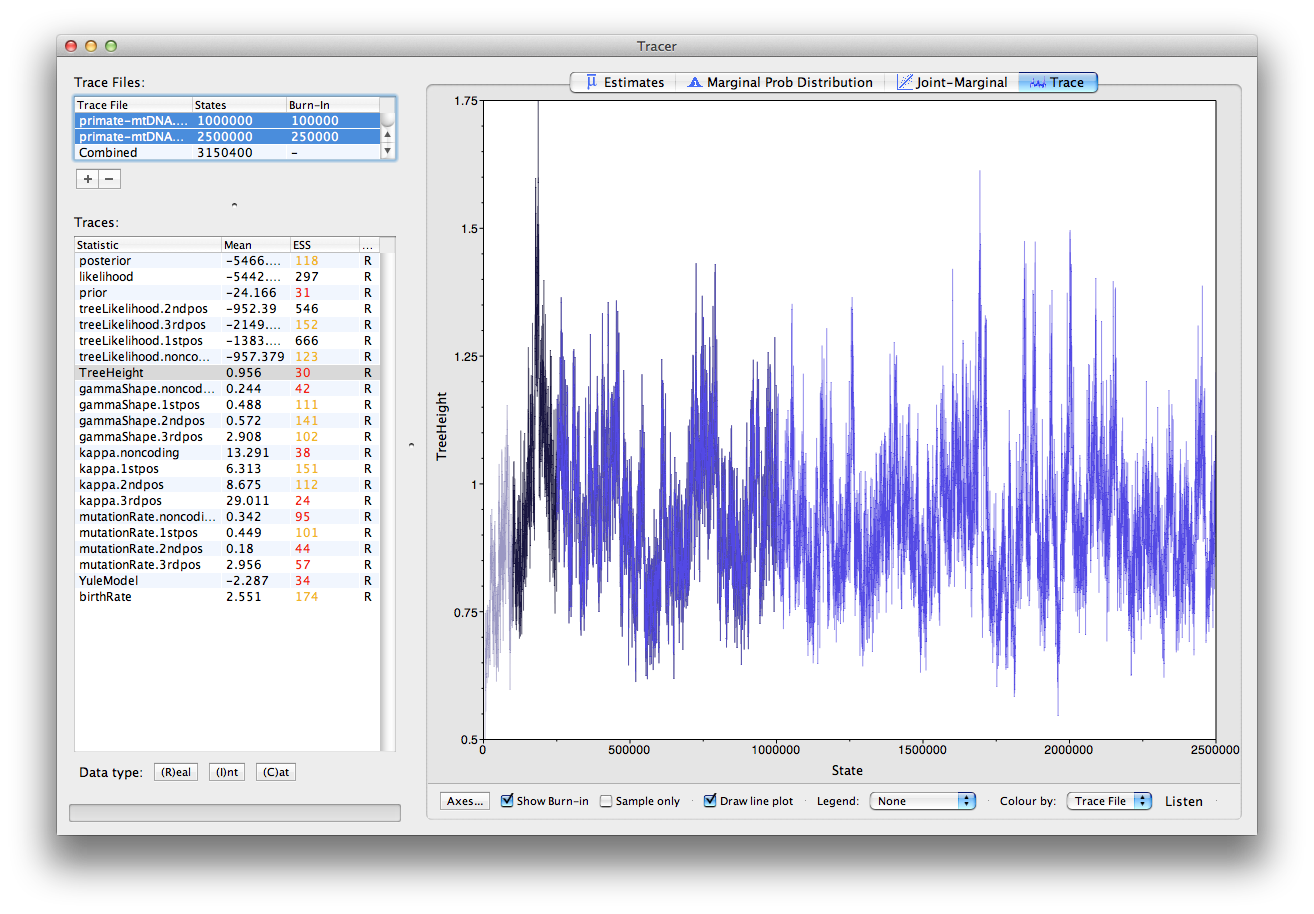
\includegraphics[width=5in]{figures/tracer_two.png}
%\caption{\small Tracer showing traces of two separate analyses ran with the same seed. The black line corresponds to the shorter run, with the beginning being coloured gray to indicate burn-in. The violet line corresponds to the longer run. With close inspection one can see that the black line, going on until 1'000'000 samples, is hidden behind the violet line, showing that if one runs the exact same analysis in BEAST2 with the same seed, the traces will be identical.}
%\label{fig:tracer_two}
%\end{figure}

\subsection{Analysing tree estimates}

Besides producing a sample of parameter estimates, BEAST2 also produces a posterior sample of phylogenetic time-trees. These need to be summarized too before any conclusions about the quality of the posterior estimate can be made.

\subsubsection{Obtaining an estimate of the phylogenetic tree}

One way to summarise the trees is by using the program TreeAnnotator. This will take the set of trees and find the best supported one. It will then annotate this representative summary tree with the mean ages of all the nodes and the corresponding 95\% HPD ranges. It will also calculate the posterior clade probability for each node. Such a tree is called the maximum clade credibility tree.

Run the TreeAnnotator program and set the \texttt{Burnin percentage} to 1\%, which will make the program ignore 1\% of the trees sampled.

\begin{framed}
Run TreeAnnotator.

Set the \texttt{Burnin percentage} to 1.
\end{framed}

The next option, the \texttt{Posterior probability limit}, specifies a limit such that if a node is found at less than this frequency in the sample of trees (i.e. has a posterior probability less than this limit), it will not be annotated. For example, setting it to 0.5 means that only nodes seen in the majority (more than 50\%) of trees will be annotated. The default value is 0, which we will leave as is, and which means that TreeAnnotator will annotate all nodes.

\begin{framed}
Leave the \texttt{Posterior probability limit} at the default value of 0.
\end{framed}

For the \texttt{Target tree type} option you can either choose a specific tree from a file or ask TreeAnnotator to find a tree in your sample. The default option which we will leave, \texttt{Maximum clade credibility tree}, finds the tree with the highest product of the posterior probability of all its nodes.

\begin{framed}
Leave the \texttt{Target tree type} at the default value of \texttt{Maximum clade credibility tree}.
\end{framed}

Next, select \texttt{Mean heights} for the \texttt{Node heights}. This sets the heights (ages) of each node in the tree to the mean height across the entire sample of trees for that clade.

\begin{framed}
Select \texttt{Mean heights} in the \texttt{Node heights} dropdown menu.
\end{framed}

Then set the \texttt{Input Tree File} to the file \texttt{.trees} file BEAST2 created as the result of the run and set the \texttt{Output File} to something like \texttt{Primates.MCC.tree}. The setup should look as shown in Figure~\ref{fig:treeannot}. You can now run the program.

\begin{framed}
Set the \texttt{Input Tree File} to the \texttt{primate-mtDNA.trees} file.

Set the \texttt{Output File} to \texttt{Primates.MCC.tree}.

Run the MCC tree generation by clocking the \texttt{Run} button.
\end{framed}

\begin{figure}[!h]
\centering
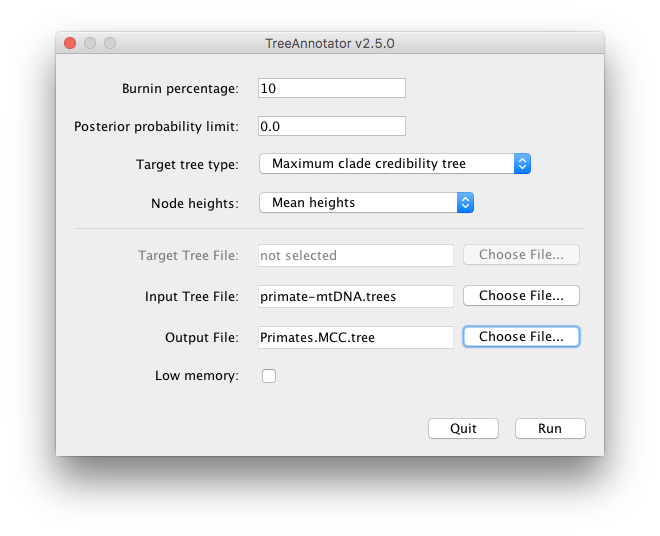
\includegraphics[width=5in]{figures/treeannot.png}
\caption{\small TreeAnnotator setup}
\label{fig:treeannot}
\end{figure}

\subsubsection{Visualising the tree estimate}

Finally, we can visualize the tree with one of the available pieces of software, such as FigTree and DensiTree.

First let us run FigTree and open the \texttt{Primates.MCC.tree} file by using \texttt{File > Open}. You can now try selecting some of the options in the control panel on the left. Try checking the \texttt{Node Bars} checkbox to get node age error bars. You will also need to expand the \texttt{Node Bars} options and select the \texttt{height\_95\%\_HPD} in the \texttt{Display} dropdown.

\begin{framed}
Run FigTree.

Open the \texttt{Primates.MCC.tree} file using \texttt{File > Open}.

Check the \texttt{Node Bars} checkbox.

Expand the \texttt{Node Bars} options and select the \texttt{height\_95\%\_HPD} in the \texttt{Display} dropdown.
\end{framed}

You can also turn on \texttt{Node Labels} and select \texttt{posterior} in the \texttt{Display} dropdown to get it to display the posterior probability for each node. You should end up with something similar to Figure~\ref{fig:figtree}.

\begin{framed}
Check the \texttt{Node Labels} checkbox.

Expand the \texttt{Node Labels} options and select the \texttt{posterior} in the \texttt{Display} dropdown.
\end{framed}

\begin{figure}[!h]
\centering
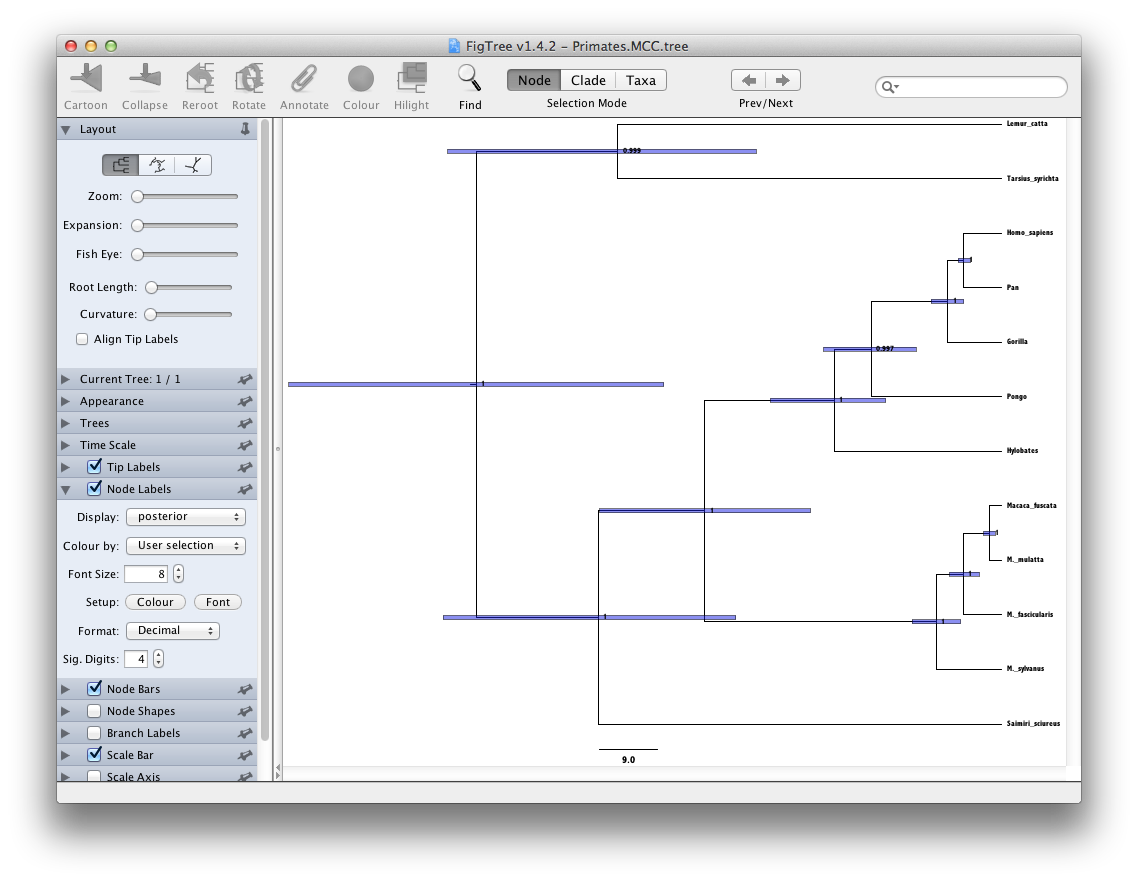
\includegraphics[width=5in]{figures/figtree.png}
\caption{\small FigTree visualisation of the estimated tree.}
\label{fig:figtree}
\end{figure}

Another program we can use is called DensiTree. DensiTree does not need a summary tree (so we do not need to run TreeAnnotator prior to using DensiTree) to be able to visualise the estimates. Run DensiTree and using \texttt{File > Load} load the .trees file. You should now see many lines corresponding to all the individual trees samples by your MCMC chain. You can also see clearly a pattern coming out. To see the pattern more clearly, expand the \texttt{Show} options and check the \texttt{Consensus Trees} to see the consensus tree of the sample.

\begin{framed}
Run DensiTree.

Open the \texttt{primate-mtDNA.trees} file using \texttt{File > Load}.

Expand the \texttt{Show} options and check the \texttt{Consensus Trees} checkbox.
\end{framed}

In order to see the support for the topology you see, select the \texttt{Central} view mode. Now expand the \texttt{Clades} menu, check the \texttt{Show clades} checkbox and the \texttt{text} checkbox for the \texttt{Support}. The tree should look as shown in Figure~\ref{fig:densitree}.

\begin{framed}
Select the \texttt{Central} view mode in the top right menu.

Expand the \texttt{Clades} menu.

Check the \texttt{Show clades} checkbox and the \texttt{text} checkbox for the \texttt{Support}.
\end{framed}

Now, select the \texttt{Help > View clades} in DensiTree menu. You should see a window that shows the different clades and their probabilities. In this particular run there is little uncertainty in the tree estimate with respect to clade grouping, as almost each clade has 100\% support.

\begin{framed}
Select \texttt{Help > View clades} and view the different clades and their probabilities.
\end{framed}

\begin{figure}[!h]
\centering
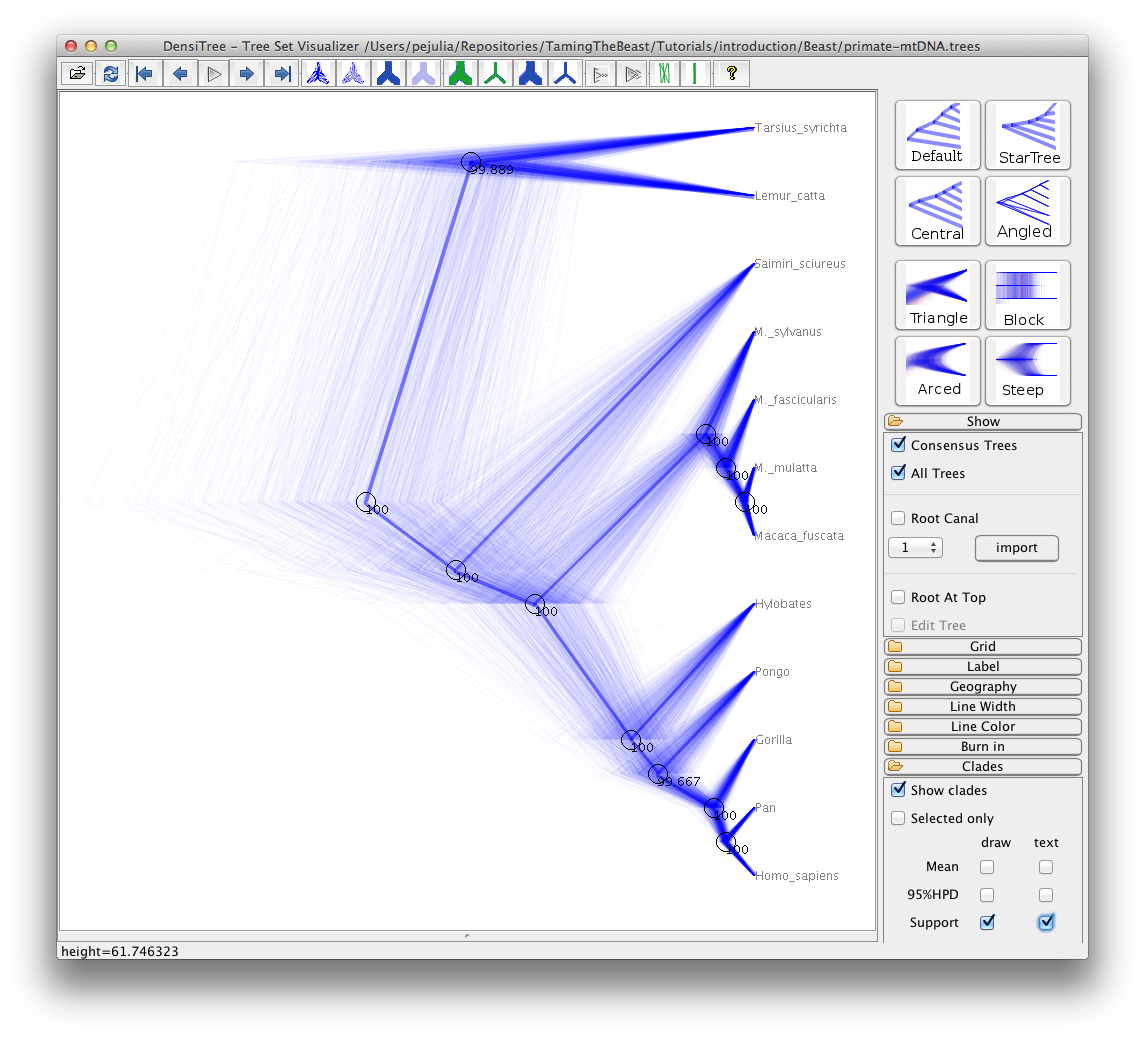
\includegraphics[width=5in]{figures/densitree.png}
\caption{\small DensiTree visualisation of the tree sample.}
\label{fig:densitree}
\end{figure}

\begin{figure}[!h]
\centering
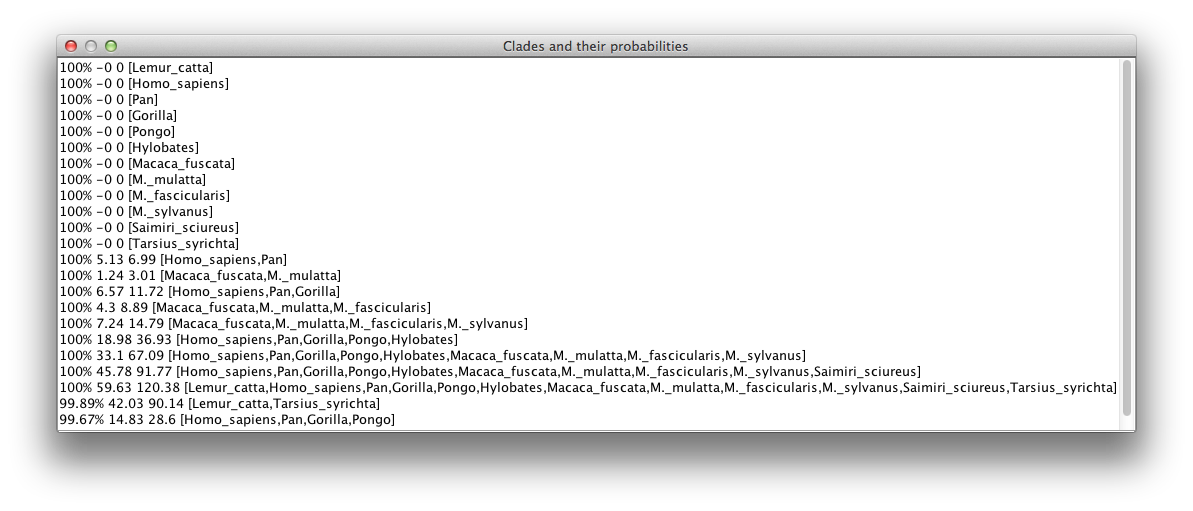
\includegraphics[width=5in]{figures/densitree_clades.png}
\caption{\small DensiTree clade probability.}
\label{fig:densitree_clades}
\end{figure}

\clearpage
\bigskip
\section{Useful Links}

\begin{itemize}
\item \href{http://www.beast2.org/book.html}{\textit{Bayesian Evolutionary Analysis with BEAST 2}}
\item BEAST 2 website and documentation: \href{http://www.beast2.org/}{http://www.beast2.org/} 
\item BEAST 1 website and documentation: \href{http://beast.bio.ed.ac.uk}{http://beast.bio.ed.ac}
\item Join the BEAST user discussion: \href{http://groups.google.com/group/beast-users}{http://groups.google.com/group/beast-users} 
\end{itemize}

\href{http://creativecommons.org/licenses/by/4.0/}{\includegraphics[scale=0.8]{figures/ccby.pdf}} This tutorial was written by \href{https://www.bsse.ethz.ch/cevo/the-group/people/person-detail.html?persid=192596}{J\={u}lija Pe\v{c}erska} and \href{https://www.bsse.ethz.ch/cevo/the-group/people/person-detail.html?persid=184671}{Veronika Bo\v{s}kov\'{a}} for the \href{https://www.bsse.ethz.ch/cevo/taming-the-beast.html}{Taming the BEAST Workshop} on applied phylogenetics and molecular evolution and is licensed under a \href{http://creativecommons.org/licenses/by/4.0/}{Creative Commons Attribution 4.0 International License}. The content is based on the \href{https://github.com/CompEvol/beast2/blob/master/doc/tutorials/DivergenceDating/DivergenceDatingTutorialv2.0.3.pdf?raw=true}{Divergence Dating Tutorial with BEAST 2.0} by Drummond, Rambaut, and Bouckaert.



Version dated: \today


\newpage

%%%%%%%%%%%%%%%%%%%%%%%%%%%%%%%%%%%%
%  REFERENCES  
%%%%%%%%%%%%%%%%%%%%%%%%%%%%%%%%%%%%

\printbibliography[heading=relevref]



\end{document}
